\documentclass[notes]{beamer}

\usepackage{listings}
\usepackage{xcolor}
\usepackage[bottom]{footmisc}

\usetheme{AnnArbor}
\usecolortheme{beaver}

\newcommand{\todo}[1]{{\color{blue}{{\bf todo: }#1}}}

\setbeamertemplate{bibliography item}{\insertbiblabel}

\lstset{ 
  backgroundcolor=\color{white},
  basicstyle=\tiny,
  breakatwhitespace=false,
  breaklines=true,
  captionpos=b,
  commentstyle=\color{green},
  deletekeywords={...},
  escapeinside={\%*}{*)},
  extendedchars=true,
  frame=single,
  keepspaces=true,
  keywordstyle=\color{blue},
  language=Python,
  morekeywords={*,...},
  numbers=left,
  numbersep=5pt,
  numberstyle=\tiny\color{gray},
  rulecolor=\color{black},
  showspaces=false,
  showstringspaces=false,
  showtabs=false,
  stepnumber=2,
  stringstyle=\color{purple},
  tabsize=2,
  title=\lstname
}

\title{PATHspider II: The Tutorial}
\author{Iain R. Learmonth}
\institute[UoA]{University of Aberdeen}

\begin{document}

\begin{frame}
\maketitle
\end{frame}

\begin{frame}
\frametitle{Active Measurement of Path Transparency}
\begin{columns}[T]
  \begin{column}{.65\textwidth}
    \begin{itemize}
    \item{Methodology:}
    \begin{enumerate}
    \item{Throw packets at the Internet}
    \item{See what happens}
    \end{enumerate}
    \item{Ideal: two-ended A/B testing}
    \item{Scalable: one-ended A/B testing}
    \item{Multiple sources: \textbf{isolate} on-path from near-target impairment}
    \end{itemize}
  \end{column}
  \begin{column}{.35\textwidth}
    \begin{figure}
      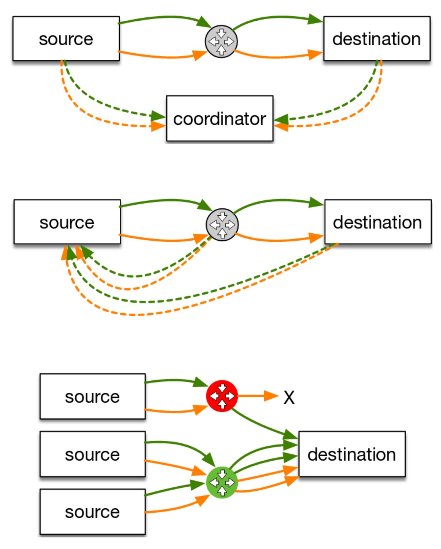
\includegraphics[width=\textwidth]{one-two-ended.png}
      \caption{One-Ended vs. Two-Ended Testing}
    \end{figure}
  \end{column}
\end{columns}
\end{frame}

\begin{frame}
\frametitle{History}
\framesubtitle{\textit{ecnspider}}
\begin{columns}[T]
  \begin{column}{.6\textwidth}
    \begin{itemize}
      \item{The original implementation supported by mPlane/RITE}
      \item{Three distinct components:}
      \begin{itemize}
        \item{DNS List Resolver}
        \item{QoF Flow Meter}
        \item{Active Traffic Generator}
      \end{itemize}
      \item{Used hardcoded \texttt{sysctl(1)} and \texttt{iptables(1)} commands
            to cause packets to be emitted with various ECN-related flags}
      \item{Source code: https://github.com/britram/ecnspider}
    \end{itemize}
  \end{column}
  \begin{column}{0.4\textwidth}
    \begin{figure}
      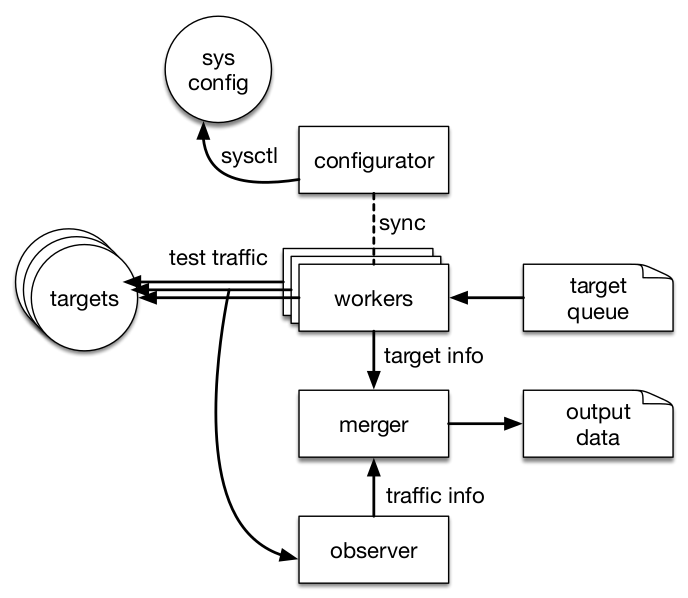
\includegraphics[width=\textwidth]{original-architecture.png}
      \caption{Original Architecture}
    \end{figure}
  \end{column}
\end{columns}
\end{frame}

\note{QoF is an IPFIX Metering and Exporting process derived from the YAF
flowmeter, designed for passive measurement of per-flow performance
characteristics.

While it was fast, it was only able to export flow properties it already knew
about, and could not be easily extended.

If you are interested in network measurement, you may still like to read about
Internet Protocol Flow Information Export (IPFIX)~\cite{rfc7011}. It was
created based on the need for a common, universal standard of export for
Internet Protocol flow information from routers, probes and other devices that
are used by mediation systems, accounting/billing systems and network
management systems to facilitate services such as measurement, accounting and
billing.}

\begin{frame}
\frametitle{History}
\framesubtitle{\textit{ecnspider} Results}
\begin{columns}[T]
  \begin{column}{.65\textwidth}
    \begin{itemize}
      \item{ECN negotiation was found to be successful for 56.17\% of hosts
	    connecting for IPv4, 65.41\% for IPv6, from the Alexa top 1 million
            list~\cite{PAM2015}}
      \item{This continues a trend ETH started observing with
            \textit{ecnspider} in 2013~\cite{PAM2013}}
    \end{itemize}
  \end{column}
  \begin{column}{.35\textwidth}
    \begin{figure}
    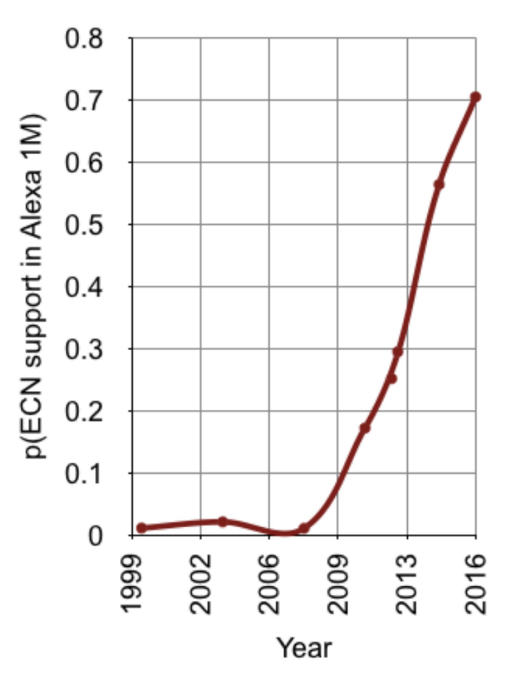
\includegraphics[width=0.9\textwidth]{ecn-trend.png}
    \caption{ECN Support in the Alexa Top 1 Million}
    \end{figure}
  \end{column}
\end{columns}
\end{frame}

\begin{frame}
\frametitle{PATHspider 1.0\footnote{https://github.com/mami-project/pathspider/tree/1.0.1}}
\begin{itemize}
\item{Architecture based closely on the original ecnspider}
\item{Generalised to support more than just ECN}
\begin{itemize}
\item{Added TCP Fast Open and DiffServ Codepoints}
\end{itemize}
\item{Still performing A/B testing, but with more A/B tests}
\item{Replaced QoF with a Python flowmeter implementation using python-libtrace}
\item{Began to develop a generalised measurement methodology for path
      transparency testing}
\item{Published at 2016 Applied Networking Research Workshop~\cite{PATHspider2016}}
\end{itemize}
\end{frame}

\begin{frame}
\frametitle{Plugin Architecture}
\begin{itemize}
\item{The plugin architecture was not as generalised as it could have been}
\item{Plugin methods:}
\begin{itemize}
\item{\texttt{config\_zero}}
\item{\texttt{config\_one}}
\item{\texttt{connect}}
\item{\texttt{post\_connect}}
\item{\texttt{create\_observer}}
\item{\texttt{merge}}
\end{itemize}
\end{itemize}
\end{frame}

\begin{frame}
\frametitle{Built-In Flowmeter}
\begin{itemize}
\item{PATHspider's built in flow meter is extensible via the plugin architecture}
\item{Using python-libtrace to dissect packets, any flow property imaginable
      can be reported back based on the raw packets:}
\begin{itemize}
\item{ECN negotiation (IP/TCP headers)}
\item{Bleaching of bits, dropping of options}
\item{Checksum recalculations}
\end{itemize}
\end{itemize}
\end{frame}

\begin{frame}
\frametitle{PATHspider 1.0 Results}
We presented some initial findings along with the publication of PATHspider
1.0~\cite{PATHspider2016}:
\begin{columns}[T]
  \begin{column}{.5\textwidth}
    Explicit Congestion Notification (ECN)

    {\tiny State of ECN server-side deployment, as measured from a Digital
           Ocean vantage point in Amsterdam on 13th June 2016:}

    \begin{table}
    \resizebox{\textwidth}{!}{%
    \begin{tabular}{ | c | c | c | c | }
    \hline
     & \textbf{IPv4} & \textbf{IPv6} & \textbf{all} \\
    \hline
    \textbf{No ECN connectivity issues} & 99.5\% & 99.9\% & 99.5\% \\
    \hline
    \textbf{ECN successfully negotiated} & 70.0\% & 82.8\% & 70.5\% \\
    \hline
    \end{tabular}}
    \end{table}

    {\tiny ECN negotiation by Alexa rank bin:}

    \begin{figure}
    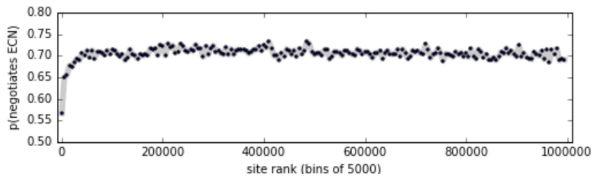
\includegraphics[width=\textwidth]{negotiation-alexa-2016.png}
    \end{figure}
  \end{column}
  \begin{column}{.5\textwidth}
    DiffServ Code Points (DSCP)

    {\tiny Initial study: 10,006 of 96,978 (10.31\%) of Alexa Top 100k websites
	   had unexpected, non-zero DSCP values. More measurement was needed to
           better characterize these anomalies.}

    TCP Fast Open (TFO)

    {\tiny Initial study: 330 IPv4 and 32 IPv6 addresses of Alexa Top 1M are
	   TFO-capable (of which 278 and 28 respectively are Google
	   properties). DDoS prevention services, enterprise firewalls, and CPE
	   tend to interfere with TFO.  More measurement was necessary to
           analyze impairments.}
  \end{column}
\end{columns}
\end{frame}

\note{Higher ranked servers tended to disable (or not support to begin with)
ECN. This is likely due to the specialised nature of services that have to
handle such large volumes of traffic. They may be using entirely custom
codebases, or are otherwise tuned and optimised.

For a more comprehensive measurement study on the use and impairments to use of DiffServ Codepoints in the Internet, see~\cite{UsableMTU2018}.}

\begin{frame}
\frametitle{PATHspider 2.0}
\begin{columns}[T]
\begin{column}{.7\textwidth}
\begin{itemize}
\item{Architecture changed to add a flow combiner}
\item{Generalised to support more than just A/B testing}
\begin{itemize}
\item{Any permutation of any number of tests}
\end{itemize}
\item{Replaced PATHspider's HTTP code with cURL}
\item{Added framework for packet forging based plugins using Scapy}
\item{Completely rewritten (in Go) target list resolver}
\item{Observer modules usable for standalone passive observation or analysis}
\item{Source code: https://github.com/mami-project/pathspider/tree/2.0.0/}
\end{itemize}
\end{column}
\begin{column}{.3\textwidth}
\begin{figure}
\includegraphics[width=\textwidth]{new-architecture.png}
\caption{New Architecture}
\end{figure}
\end{column}
\end{columns}
\end{frame}

\note{The combiner thread holds a table of merged flows and waits for
      $\vert flows\vert = \vert jobs\vert$. Conditions are generated based on the
      combined flows.}

\begin{frame}
\frametitle{Plugin Types}
\begin{itemize}
\item{Synchronised (traditional ecnspider)}
\begin{itemize}
\item{ECN, DSCP}
\end{itemize}
\item{Desynchronised (traditional ecnspider, no configurator)}
\begin{itemize}
\item{TFO, H2, TLS NPN/ALPN}
\end{itemize}
\item{Forge (new in PATHspider 2.0!)}
\begin{itemize}
\item{Evil Bit, UDP Zero Checksum, UDP Options}
\end{itemize}
\item{Single (new, and fast)}
\begin{itemize}
\item{Various TCP Options}
\end{itemize}
\end{itemize}
\end{frame}

\note{The desynchronized plugins will run more quickly than synchronized
      plugins while still using the real network stack. Forge plugins will run
      slower as there is overhead in the Scapy packet generation that doesn't
      exist in optimised kernel stacks.}

\begin{frame}
\frametitle{Connection Helpers}
\begin{itemize}
\item{Instead of writing client code, use the code that already exists}
\item{In the \texttt{pathspider.helpers} module:}
\begin{itemize}
\item{DNS (dnslib)}
\item{HTTP/HTTPS (pycURL)}
\item{TCP (Python socket)}
\end{itemize}
\item{For synchronised plugins, just use the helper}
\item{For desycnhronised plugins, the helpers are customisable, e.g. cURL
      helpers accept arbitrary CURLOPTs}
\end{itemize}
\end{frame}

\note{\todo{Pointer to the pycURL documentation, and talk about upstreaming
            CURLOPTs}}

\begin{frame}
\frametitle{Synchronized Plugin}
\todo{Write this}
\end{frame}

\begin{frame}
\frametitle{Desynchronized Plugin}
\todo{Write this}
\end{frame}

\begin{frame}
\frametitle{Forge Plugin}
\todo{Write this}
\end{frame}

\begin{frame}
\frametitle{Single Plugin}
\todo{Write this}
\end{frame}

\begin{frame}[fragile]
\frametitle{Observer Modules}
\begin{itemize}
\item{While these used to be part of plugins in PATHspider 1.0, they are now independent and so can be reused across multiple plugins:}
\begin{itemize}
\item{BasicChain, DNSChain, DSCPChain, ECNChain, EvilChain, ICMPChain, TCPChain, TFOChain}
\end{itemize}
\item{These can also be used together, limiting each chain to just a single layer and letting the combiner produce conditions}
\item{Chains can produce information to be consumed by other chains later in the list}
\item{These can be used independently of a PATHspider measurement:}
\end{itemize}
\begin{lstlisting}[caption={Running the PATHspider Observer independently}]
irl@z~$ pspdr observe tcp ecn
\end{lstlisting}
\end{frame}

\begin{frame}
\frametitle{Target List Resolution}
\begin{itemize}
\item{Hellfire is a parallelised DNS resolver. It is written in Go and for the purpose of generating input lists to PATHspider, though may be useful for other applications}
\item{Can use many sources for inputs:}
\end{itemize}
\begin{columns}[T]
\begin{column}{.7\textwidth}
\begin{itemize}
\item[]{
\begin{itemize}
\item{Alexa Top 1 Million Global Sites}
\item{Cisco Umbrella 1 Million}
\item{Citizen Lab Test Lists}
\item{OpenDNS Public Domain Lists}
\item{Comma-Seperated Values Files}
\item{Plain Text Domain Lists}
\end{itemize}}
\end{itemize}
\end{column}
\begin{column}{.3\textwidth}

\includegraphics[width=.8\textwidth]{hellfire-logo.png}
\end{column}
\end{columns}
\begin{itemize}
\item{More on this later}
\end{itemize}
\end{frame}

\begin{frame}
\frametitle{Packet Forging}
\begin{itemize}
\item{PATHspider uses the Scapy library for Python for packet forging}
\item{This is the most flexible method of creating new measurement plugins for
      PATHspider}
\end{itemize}
\end{frame}

\begin{frame}
\frametitle{Make a Packet}
\begin{itemize}
\item{Scapy packets are constructed layer by layer}
\item{While you can specify raw bytes, Scapy provides a number of useful
      classes for common protocols, which makes things a lot easier}
\end{itemize}
\end{frame}

\begin{frame}[fragile]
\frametitle{Make a Packet}
\begin{itemize}
\item{\tiny Scapy must be launched with \texttt{sudo} as we will need to use
             ``raw" sockets to emit forged packets.}
\item{\tiny Note also the command is \texttt{scapy\textit{3}}, to ensure we
             are running the Python 3 version.}
\end{itemize}
\begin{lstlisting}[caption={Launching Scapy}]
irl@z:~$ sudo scapy3
                                      
                     aSPY//YASa       
             apyyyyCY//////////YCa       |
            sY//////YSpcs  scpCY//Pp     | Welcome to Scapy
 ayp ayyyyyyySCP//Pp           syY//C    | Version 2.4.0
 AYAsAYYYYYYYY///Ps              cY//S   |
         pCCCCY//p          cSSps y//Y   | https://github.com/secdev/scapy
         SPPPP///a          pP///AC//Y   |
              A//A            cyP////C   | Have fun!
              p///Ac            sC///a   |
              P////YCpc           A//A   | We are in France, we say Skappee.
       scccccp///pSP///p          p//Y   | OK? Merci.
      sY/////////y  caa           S//P   |             -- Sebastien Chabal
       cayCyayP//Ya              pY/Ya   |
        sY/PsY////YCc          aC//Yp 
         sc  sccaCY//PCypaapyCP//YSs  
                  spCPY//////YPSps    
                       ccaacs         
                                       using IPython 5.5.0
>>> 
\end{lstlisting}
\end{frame}

\begin{frame}[fragile]
\frametitle{Make a Packet}
\framesubtitle{IPv4 Header - Create and Dissect}
\begin{lstlisting}[caption={Creating and Dissecting an IPv4 Header}]
>>> IP()
<IP  |>
>>> i = IP()
>>> i.summary()
'127.0.0.1 > 127.0.0.1 hopopt'
>>> i.display()
###[ IP ]### 
  version= 4
  ihl= None
  tos= 0x0
  len= None
  id= 1
  flags= 
  frag= 0
  ttl= 64
  proto= hopopt
  chksum= None
  src= 127.0.0.1
  dst= 127.0.0.1
  \options\
\end{lstlisting}
\end{frame}

\begin{frame}[fragile]
\frametitle{Make a Packet}
\framesubtitle{IPv4 Header - Customize}
\begin{lstlisting}[caption={Customizing an IPv4 Header\footnote{These IP addresses have been reserved for use in documentation and examples, and should not be used publicly\cite{rfc5737}.}}]
>>> i = IP(src="192.0.2.1",dst="198.51.100.1", ttl=10)
>>> i
<IP  ttl=10 src=192.0.2.1 dst=198.51.100.1 |>
>>> i.summary()
'192.0.2.1 > 198.51.100.1 hopopt'
>>> i.display()
###[ IP ]### 
  version= 4
  ihl= None
  tos= 0x0
  len= None
  id= 1
  flags= 
  frag= 0
  ttl= 10
  proto= hopopt
  chksum= None
  src= 192.0.2.1
  dst= 198.51.100.1
  \options\
\end{lstlisting}
\end{frame}

\begin{frame}[fragile]
\frametitle{Make a Packet}
\framesubtitle{IPv4 Header - Bonus: Export a Dissection}
\begin{lstlisting}[caption={Create a PDF Export of a Dissection of the IP Header}]
>>> i.pdfdump()
\end{lstlisting}

\begin{figure}
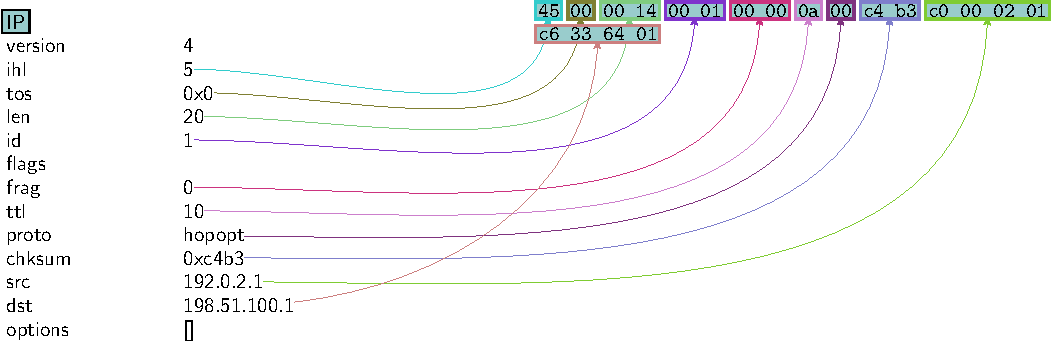
\includegraphics[width=0.7\textwidth]{ip_dissect}
\caption{PDF Export of IP Header Dissection}
\end{figure}
\end{frame}

\begin{frame}[fragile]
\frametitle{Make a Packet}
\framesubtitle{TCP Header: Create and Dissect}
\begin{lstlisting}[caption={Creating and Dissecting a TCP Header}]
>>> TCP()
<TCP  |>
>>> t = TCP()
>>> t.summary()
'TCP ftp_data > http S'
>>> t.display()
###[ TCP ]### 
  sport= ftp_data
  dport= http
  seq= 0
  ack= 0
  dataofs= None
  reserved= 0
  flags= S
  window= 8192
  chksum= None
  urgptr= 0
  options= []

\end{lstlisting}
\end{frame}

\begin{frame}[fragile]
\frametitle{Make a Packet}
\framesubtitle{TCP Header: Customizing}
\begin{lstlisting}[caption={Customizing a TCP Header}]
>>> t = TCP(dport=443)
>>> t
<TCP  dport=https |>
>>> t.summary()
'TCP ftp_data > https S'
>>> t.display()
###[ TCP ]### 
  sport= ftp_data
  dport= https
  seq= 0
  ack= 0
  dataofs= None
  reserved= 0
  flags= S
  window= 8192
  chksum= None
  urgptr= 0
  options= []
\end{lstlisting}
\end{frame}

\begin{frame}
\frametitle{Make a Packet}
\frametitle{Modifying a Packet}
\todo{Modify a packet}
\end{frame}

\begin{frame}[fragile]
\frametitle{Make a Packet}
\framesubtitle{Sticking the Pieces Together}
\begin{itemize}
\item{The \texttt{/} operator is used to join layers together.}
\item{Scapy will automatically set fields, such as the IP Protocol field, when
      you do this.}
\item{When dissecting, Scapy will automatically choose the dissector to use
      based on fields such as the IP Protocol field.}
\end{itemize}
\begin{lstlisting}[caption={Sticking the IP and TCP Headers Together}]
>>> p=i/t
>>> p.summary()
'IP / TCP 192.0.2.1:ftp_data > 198.51.100.1:https S'
>>> p.display()
    [... output snipped ...]
\end{lstlisting}
\end{frame}

\begin{frame}[fragile]
\frametitle{Make a Packet}
\framesubtitle{View in Wireshark}
\begin{lstlisting}[caption={Exporting a PCAP File from Scapy}]
>>> wrpcap("/tmp/scapy.pcap", [p])
\end{lstlisting}
\begin{figure}
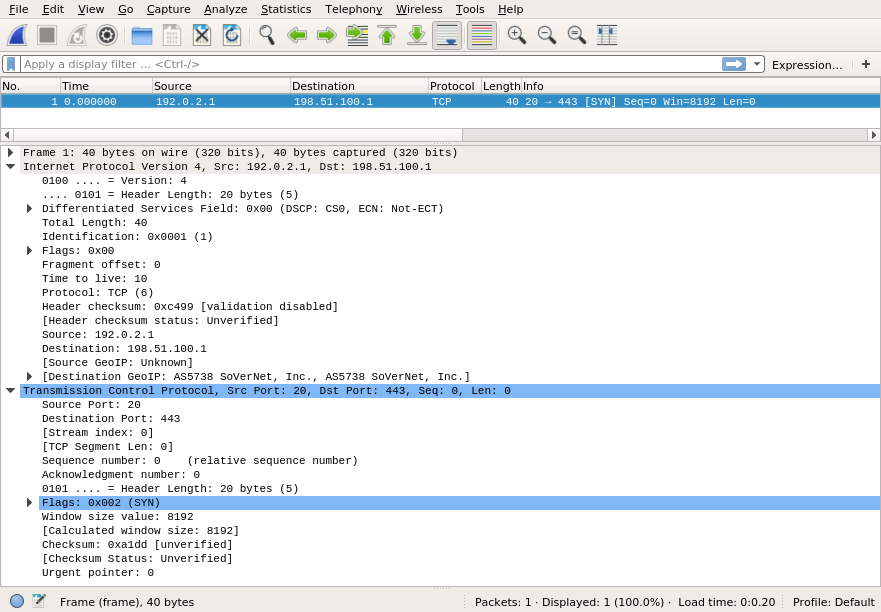
\includegraphics[width=0.5\textwidth]{scapy-wireshark.png}
\caption{Dissection of the packet created in Scapy, in Wireshark}
\end{figure}
\end{frame}

\begin{frame}[fragile]
\frametitle{Send a Packet}
\begin{itemize}
\item{The \texttt{sr1()} function sends a single packet, and returns a single
      packet if a reply is received.}
\item{Start Wireshark capturing before executing the \texttt{sr1()} function.}
\end{itemize}
\begin{lstlisting}[caption={Create and Send an IP/TCP Packet}]
>>> p=IP(dst="139.133.210.32")/TCP()
>>> a=sr1(p)
Begin emission:
.Finished sending 1 packets.
*
Received 2 packets, got 1 answers, remaining 0 packets
>>> a
<IP  version=4 ihl=5 tos=0x0 len=44 id=0 flags=DF frag=0 ttl=47 proto=tcp chksum=0xa98d src=139.133.210.32 dst=172.22.152.130 options=[] |<TCP  sport=http dport=ftp_data seq=3081101820 ack=1 dataofs=6 reserved=0 flags=SA window=29200 chksum=0xe9c7 urgptr=0 options=[('MSS', 1452)] |<Padding  load=':v' |>>>
>>> a.summary()
'IP / TCP 139.133.210.32:http > 172.22.152.130:ftp_data SA / Padding'
\end{lstlisting}
\end{frame}

\begin{frame}
\frametitle{Evil Bit}
\begin{quote}
The evil bit is a fictional \textbf{IPv4 packet header field} proposed in RFC 3514 \cite{rfc3514}, a humorous April Fools' Day RFC from 2003 authored by Steve Bellovin. The RFC recommended that the last remaining unused bit, the "Reserved Bit," in the IPv4 packet header be used to indicate whether a packet had been sent with malicious intent, thus making computer security engineering an easy problem \textemdash~simply ignore any messages with the evil bit set and trust the rest.
\end{quote}
\hfill -- Wikipedia
\end{frame}

\note{If you enjoy the concept of the evil bit, you may like to also check out
      \cite{rfc5841}: TCP Option to Denote Packet Mood. For example happy
      packets which are happy because they received their ACK return packet
      within less than 10ms. Or the Sad Packets which are sad because they faced
      retransmission rates greater than 20\% of all packets sent in a session.}

\begin{frame}[fragile]
\frametitle{Evil Bit}
\framesubtitle{Setting the Evil Bit with Scapy}
\begin{itemize}
\item{The flags in the IP header are just an attribute you can modify:}
\end{itemize}
\begin{lstlisting}[caption={Setting the Evil Bit on an IPv4 Header with Scapy}]
>>> i = IP()
>>> i.flags = 'evil'
\end{lstlisting}
\end{frame}

\begin{frame}
\frametitle{PATHspider Plugins}
\framesubtitle{Directory Layout}
\todo{Write this}
\end{frame}

\begin{frame}[fragile]
\frametitle{PATHspider Plugins}
\framesubtitle{ForgeSpider}
\begin{lstlisting}[caption={Outline for Evil Bit plugin using ForgeSpider}]
class EvilBit(ForgeSpider, PluggableSpider):

    name = "evilbit"
    description = "Evil bit connectivity testing"
    version = "0.0.0"
    chains = [...]
    connect_supported = [...]
    packets = 2

    def forge(self, job, seq):
        ...
\end{lstlisting}
\end{frame}

\begin{frame}
\frametitle{PATHspider Plugins}
\framesubtitle{Forging the Packets}
\todo{Write this}
\end{frame}

\begin{frame}
\frametitle{PATHspider Plugins}
\framesubtitle{Testing Packet Forging}
\todo{Write this}
\end{frame}

\begin{frame}
\frametitle{PATHspider Plugins}
\framesubtitle{The Observer}
\todo{Write this}
\end{frame}

\begin{frame}
\frametitle{PATHspider Plugins}
\framesubtitle{Library Observer Functions}
\todo{Write this}
\end{frame}

\begin{frame}
\frametitle{PATHspider Plugins}
\framesubtitle{Observing the Evil Bit}
\todo{Write this}
\end{frame}

\begin{frame}
\frametitle{PATHspider Plugins}
\framesubtitle{Putting it Together}
\todo{Write this}
\end{frame}

\begin{frame}
\frametitle{PATHspider Plugins}
\framesubtitle{Adding a Flow Combiner}
\todo{Write this}
\end{frame}

\begin{frame}
\frametitle{PATHspider Plugins}
\framesubtitle{Running it For Real}
\todo{Write this}
\end{frame}

\begin{frame}
\frametitle{Target Lists}
\framesubtitle{Types of Targets}
\todo{Write this}
\end{frame}

\begin{frame}[fragile]
\frametitle{Target Lists}
\framesubtitle{Using \textit{hellfire}}
\begin{lstlisting}[caption={\textit{hellfire}'s Usage Help}]
irl@z:~$ hellfire
Usage:
  hellfire --topsites [--file=<filename>] [--output=<individual|array|oneeach>] [--type=<host|ns|mx>] [--canid=<canid address>]
  hellfire --cisco [--file=<filename>] [--output=<individual|array|oneeach>] [--type=<host|ns|mx>] [--canid=<canid address>]
  hellfire --citizenlab [--country=<cc>|--file=<filename>] [--output=<individual|array|oneeach>] [--type=<host|ns|mx>] [--canid=<canid address>]
  hellfire --opendns [--list=<name>|--file=<filename>] [--output=<individual|array|oneeach>] [--type=<host|ns|mx>] [--canid=<canid address>]
  hellfire --csv --file=<filename> [--output=<individual|array|oneeach>] [--type=<host|ns|mx>] [--canid=<canid address>]
  hellfire --txt --file=<filename> [--output=<individual|array|oneeach>] [--type=<host|ns|mx>] [--canid=<canid address>]
\end{lstlisting}
\begin{lstlisting}[caption={Start Resolving the Cisco Umbrella List}]
irl@z~$ hellfire --cisco
\end{lstlisting}
\end{frame}

\begin{frame}
\frametitle{Target Lists}
\framesubtitle{Using \textit{canid} for Additional Information}
\todo{Write this}
\end{frame}

\begin{frame}
\frametitle{Target Lists}
\framesubtitle{Resolving for Real}
\todo{Write this}
\end{frame}

\begin{frame}
\frametitle{Explicit Congestion Notification}
\framesubtitle{Using the Built-In Plugin}
\todo{Write this}
\end{frame}

\begin{frame}
\frametitle{Simple Analysis with PATHspider}
\end{frame}

\begin{frame}
\frametitle{More Complex Analysis}
\begin{center}
{\LARGE Up next: \\
Path Transparency Observatory (PTO)} \\
Don't delete your PATHspider results, you'll need them in the next session.
\end{center}
\end{frame}

\begin{frame}[allowframebreaks]
\frametitle{References}
\bibliographystyle{plain}
\bibliography{pathspider-tutorial,rfc}
\end{frame}

\end{document}
